\section{Ejercicios}
\subsection{Range query circle}
Implemente la función range\_query\_circle del KD-Tree, esta vez el range representa un círculo.
\begin{lstlisting}[language=c++,
                   directivestyle={\color{black}}
                   emph={int,char,double,float,unsigned},
                   emphstyle={\color{blue}}
                  ]
function rangeQueryCircle(node, puntoConsulta, kpoints, radio, depth = 0) {
  if (!node) return null;

  var subTree1 = node.left;
  var subTree2 = node.right;

  if (puntoConsulta[depth%k] >= node.point[depth%k]) {
    subTree1 = node.right;
    subTree2 = node.left;
  }

  masCercano(point, rangeQueryCircle(subTree1, puntoConsulta, kpoints, radio, depth + 1), node.point);

  if (distanceSquared(puntoConsulta, node.point) < radio) {
    node.point.push(distanceSquared(puntoConsulta, node.point));
    kpoints.push(node.point);
  }

  if (radio >= Math.abs(puntoConsulta[depth%k] - node.point[depth%k])) {
    masCercano(puntoConsulta, rangeQueryCircle(subTree2, puntoConsulta, kpoints, radio, depth + 1), node.point);
  }
}
\end{lstlisting}

\begin{figure}[H]
  \centering
  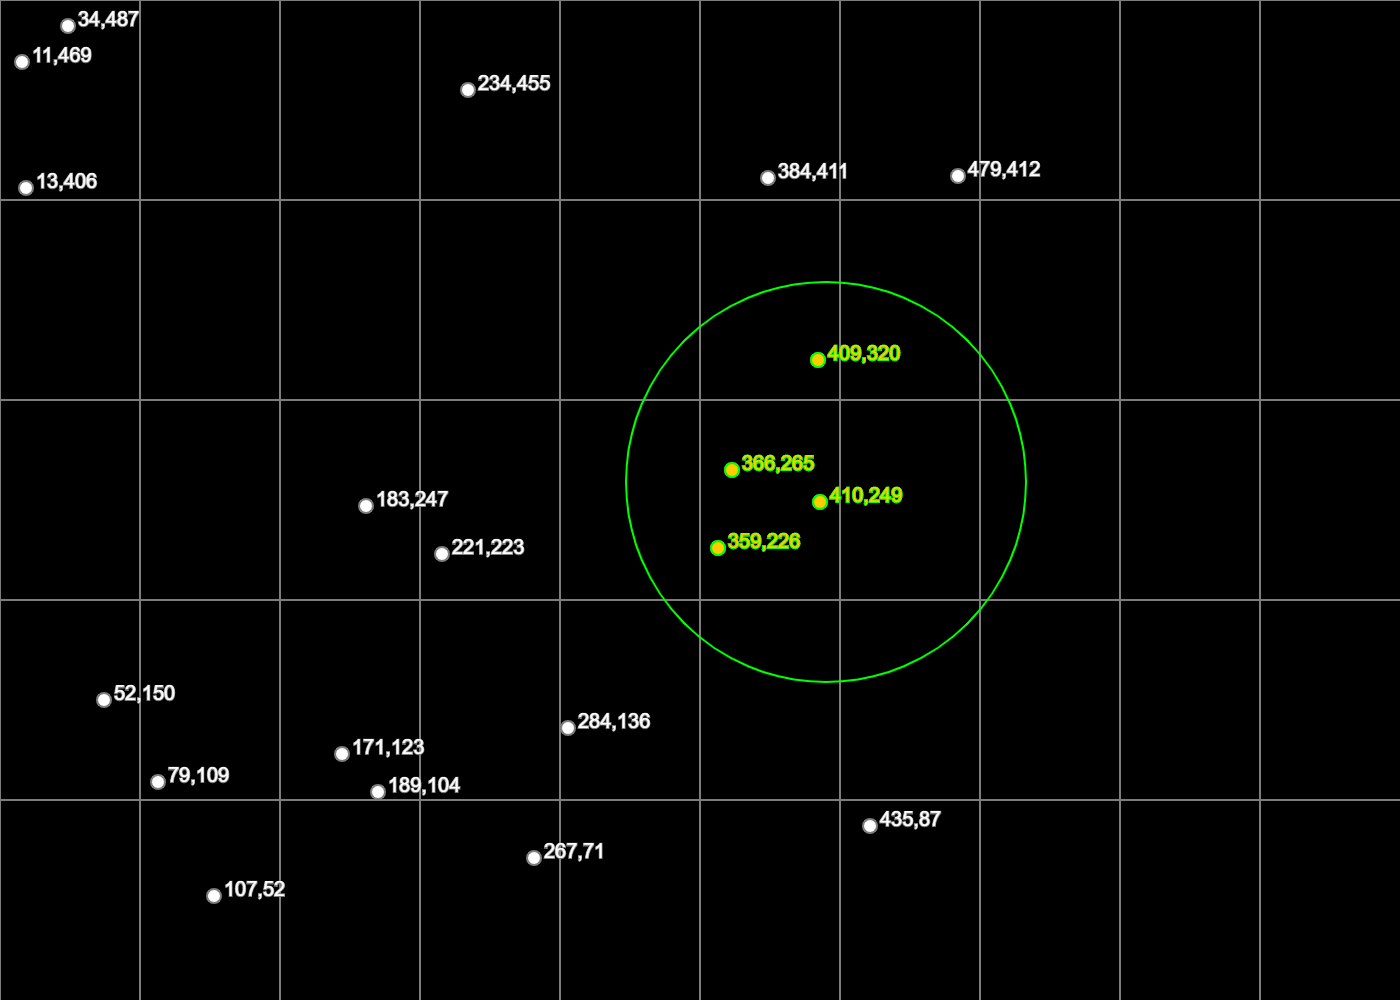
\includegraphics[width=0.8\textwidth]{images/7b.png}
  \label{fig:act-7b}
\end{figure}

